\chapter{Eksperymenty}
\section{Metodologia}
Testy przeprowadzono przy użyciu skryptu zawartego w repozytorium wosedona. Skrypt \verb|evaluation-kpwr.py| wymaga do swojego działania połączenia z bazą danych Słowosieci. Na wejście skryptu podawany jest wcześniej przetworzony przez wosedon, anotowany tekst. Wymóg anotowanego tekstu jest spowodowany tym, że musi istnieć podstawa, na której zostanie określona poprawność ujednoznaczniania. Testy wykonano na wybranych wcześniej pięciu plikach, które zawierają najwięcej wieloznacznych wyrazów, tak aby pliki wynikowe miały jak najwięcej przetworzonych wyrazów. Każdy z siedmiu zaimplementowanych algorytmów został uruchomiony na tych pięciu plikach i już zbiorczo oznaczono ilość poprawnie ujednoznacznionych wyrazów. Do usprawnienia testowania implementacji posłużono się trzema skryptami: \verb|runDocker| - uruchamiający kontener Dockera, \verb|runWosedon| uruchamiający wosedon na kolejnych algorytmach na wszystkich wybranych plikach oraz \verb|runTests|, który przetwarzał wyniki poprzedniego skryptu i oznaczał poprawnie ujednoznacznione wyrazy.
\section{Wyniki}
Poniżej przedstawiono wyniki przeprowadzonych eksperymentów. 

\begin{table}[H]
\centering
\caption{My caption}
\label{my-label}
\begin{tabular}{llll}
Nazwa           & Ilość poprawnych & Ilość niejednoznacznych & Dokładność \\
PageRank        & 39               & 145                     & 0.269      \\
Betweenness     & 61               & 145                     & 0.421      \\
Closeness       & 47               & 145                     & 0.324      \\
Eigenvector     & 44               & 145                     & 0.303      \\
Katz            & 43               & 145                     & 0.297      \\
Hits(Authority) & 45               & 145                     & 0.310      \\
Hits(Hubs)      & 43               & 145                     & 0.297     
\end{tabular}
\end{table}

\begin{figure}[H]
	\centering
		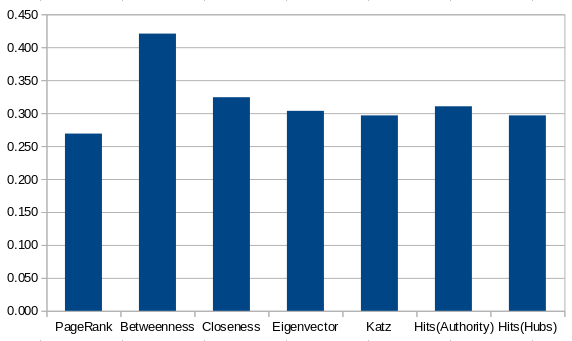
\includegraphics[width=0.75\linewidth]{img/results.png}
	\caption[Wyniki poszczególnych metod.]{Wyniki poszczególnych metod.}
	\label{fig:binary}
\end{figure}